\chapter{Music analysis techniques: state of the art} 
\label{Chapter2} 

\lhead{Chapter 2. \emph{Music analysis techniques: state of the art}} 
The main subject of MIR regards the \textit{extraction and inference of musically meaningful features, indexing of music} (through these features) and the development of \textit{search and retrieval schemes} \cite{downieMIR}. In other terms, the main target of MIR is to make all the information regarding music over the world easily accessible to the user \cite{downieMIR}. During the last two decades, several approaches have been developed, which mainly differ in the nature of the features they deal with. The main categories of sources from which features are extracted are generally considered to be the following ones: \textit{music content}, \textit{music context}, \textit{user properties} and \textit{user context} \cite{gomez14}. \textit{Music content} data deals with aspects that are directly inferred by the audio signal (such as melody, rhythmic structure, timbre) while \textit{music context} data refers to aspects that are not directly extracted from the signal but are strictly related to it (for example label \cite{pachet00}, artist and genre information \cite{perfe11} \cite{aizenberg12}, year of release \cite{vangulik05}, lyrics \cite{coelho13} and semantic labels). Regarding the user, the difference between \textit{user context} and \textit{user properties} data lies on the stability of aspects of the user himself. The former deal with aspects that are subject to frequent changes (such as mood or social context), while the latter refer to aspects that may be considered constant or slowly changing, for instance his music taste or education \cite{gomez14}. \\In this chapter, we will focus on the differences between \textit{music content} and \textit{music context} data. 


\section{Metadata}
By metadata we mean all the descriptors about a track that are not based on the audio content\footnote{We recall again that there is a lack of agreement on the use of the term metadata; elsewhere it could be used with a different meaning, for instance it may indicate all the data extracted from the audio signal itself.}. Therefore, they are not directly extracted from the audio signal but rather from external sources. They began to be deeply studied since the early 2000s, when first doubts about an upper threshold of the performance of audio content analysis systems arised \cite{aucou04}. Researchers then started exploring the possibility of performing retrieving tasks on written data that is related to the artist or to the piece. \\At first, the techniques were adapted from the Text-IR ones, but it was immediately clear that retrieving music is fairly more complex than retrieving text for several reasons:
\begin{itemize}
\item If metadata are used in a music recommendation system, they should take into account also the musical taste of the user who performed the query.
\item Text documents are in general able to provide information about its content. The user who performs the query in the hope of retrieving a particular text generally has a good idea of how to form his query. For instance, in \cite{orio06} Orio provides the example that if a user is looking for a text that is somehow linked to or setted in a tempest, he could just query ``tempest''. On the other hand, music's abstractness makes it very hard for the user to formalize in words a precise query in order to retrieve audio. 
\end{itemize}
As a consequence of this fact, it is generally believed that music characteristics can be described only in musical terms \cite{orio06}. Yet the task of describing music remains hard, for musical terms are mainly referred to structural features rather than the content, and therefore terms like \textit{concerto} or \textit{ballad} are not useful to discriminate among the different hundreds or thousands of concerti or ballads \cite{orio06}. \\ 
During last years, many techniques exploiting metadata have been developed; they may differ both in the sources used for retrieving data and in the way of computing a similarity score, and clearly the performance of a system using metadata for similarity computation is highly affected by both of these factors. Sources may include \cite{bogdanov13}:
\begin{itemize}
\item Manual annotation: description provided by experts; they may be referred to genre, mood, instrumentation, artist relations.
\item Collaborative filtering data: data indirectly provided by users of web communities, in the form of user ratings or listening behaviour information.
\item Social tags: data directly provided by users of social network of music (such as \textit{Last.fm}\footnote{\url{http://last.fm}}) or social games.
\item Information automatically mined from the Web. Sources in these cases may include web-pages related to music or microblogs (for instance the very popular \texit{Twitter}).
\end{itemize}
 The availability of some of them greatly depends on the size of the music collection under consideration; for instance, as manual expert annotations might be very accurate, they would be extremely costly and probably infeasible on large collections \cite{Szyma09}. In contrast, collaborative filtering data may be the most studied technique, given that it has already been intensively used in other different fields, for instance in movie recommendation. It is the predominant approach in the field of Recommender Systems (RS) \cite{jannach12} and is mainly focused on user ratings, generally leading to better results \cite{green09}. However, some concerns are related to this technique. First, collaborative filtering approaches have not been designed to be used for playlist generation, but mainly for recommending artists or music. Second, the availibility of datasets for user ratings in the field of music is very limited compared to other fields, and research is often based on very small samples \cite{liu09}. Regarding listening behaviour information, they might be inaccurate for they don't keep track of song durations and of the user activities while listening to music \cite{jawaheer10}. In addition, there's no way of collecting negative feedback (\textit{dislikes}) through them and, more in general, listening to a specific song doesn't necessarily imply liking that song \cite{bogdanov13}. \\Sources are also picked in relation to the subject of the research or of the system, that may be for example a recommendation or a similarity computation system. At this point, it's important to highlight the difference between the two of them: a recommendation system not only has to find similar music, but has also to take into account the personal taste of the user, and therefore it's generally considered as a basic tool to produce recommendation \cite{celma08}. In any case, the terms ``similarity'' and ``recommendation'' cannot be substituted, given that a good similarity computation system doesn't necessarily equate to a good recommendation system \cite{mcnee06}. 
 The computation of similarity may happen through a Vector Space Model (a technique adapted from the Text-IR) and co-occurence analysis. In the next subsections we will briefly explain the characteristics and the performance of these techniques.

\subsection{Vector Space Model} 
The main idea of this technique lies on building a bag-of-words representation \footnote{A bag-of-words can be basically seen as an extension of a programming language ``dictionary'': it collects words (that sometimes may just be an abstraction of much more complex features, such as computer vision descriptors) from a document, and then computes the frequency with which each of them appears in the document. Two different documents are considered similar if they contain the same or similar words with a comparable frequency.} of a retrieved document, and then computing a term weight vector for each document. It's a frequently used technique in Text-IR (and in Computer Vision) which can safely be used when retrieving web pages related to music, in an attempt of computing similarity. In \cite{whitman02}, one of the first work in this field, Whitman and Lawrence provided an analysis of this kind on music-related web pages retrieved with the queries (to the \textit{Google} search engine) ``artist'' \texttt{music review} and ``artist'' \texttt{genre style}, where words such as music and review where added to improve the chances of automatically retrieving webpages related to music. After downloading the pages, the authors apply a Part-of-Speech\footnote{Software or algorithm for automatically assign each word in a text to a speech.} tagger to assign each word to its suited test set. Similarity between pairs of artists is then computed on the tf-idf (term frequency - inverse document frequency) vectors of the respective artists. In general, the tf-idf assigns more weight to words that occur frequently in a specific document but rarely in others \cite{musicdatamining}. This approach has later been refined, by applying better filtering to the corpus of the page (in order to consider only significant words) and with different similarity measures. The use of Vector Space Model has not been limited to webpages. For instance, it has been applied to microblogs (specifically Twitter) in \cite{schedl12}, achieving a mean average precision (MAP) of 64\% on a collection of 224 artists. Interestingly enough, results of more than 23000 single experiments showed that:
\begin{itemize}
\item Queries composed only by the artist name performed best, while adding other keywords showed a decrease in accuracy.
\item Highest MAP values are achieved without filtering the corpus of the webpage (thus increasing the computational costs)
\end{itemize}
Vector Space Model has been used also with collaborative tags and games with a purpose. Collaborative tags are small annotation (usually just one or two words) created by users of social music platform, such as \textit{Last.fm} of \textit{MusicStrands}\footnote{\url{http://music.strands.com}}. The main advantage of these tags over the microblog data lies in the limited dictionary used for indexing and in the meaningfulness of these tags; in other words, tags are generally less dispersive, less noisy and more musically meaningful. Furthermore, tags are available not only at artist level, but also at the level of albums or tracks. On the other hand, they require a large and active user community. In this kind of community, moreover, the phenomenon of ``popularity bias'' is more frequent: much more data is available for popular tracks and artists, while no data at all might be found for artists in the \textit{long tail}. If this kind of data is used inside a music recommendation system, a further phenomenon of ``the rich gets richer'' may happen, as more popular songs are more subject to be recommended and therefore will be tagged by even more users. Another problem with tags of \textit{Last.fm} is that many of them are irrelevant to create a descriptive artist or song profile \cite{gomez14}, as personal and subjective tags such as ``love'' or ``favorite'' may be found. This problem can be solved with the use of data coming from games with a purpose (for instance \textit{TagATune}\footnote{\url{http://musicmachinery.com/tag/tagatune/}}), that are usually sources of much more meaningful data. In \textit{TagATune}, two players are played a song, which could be either the same or different: they have to understand as soon as possible (in order to get a higher score) if the some they're being played it's the same. 

\begin{figure}
\centering
    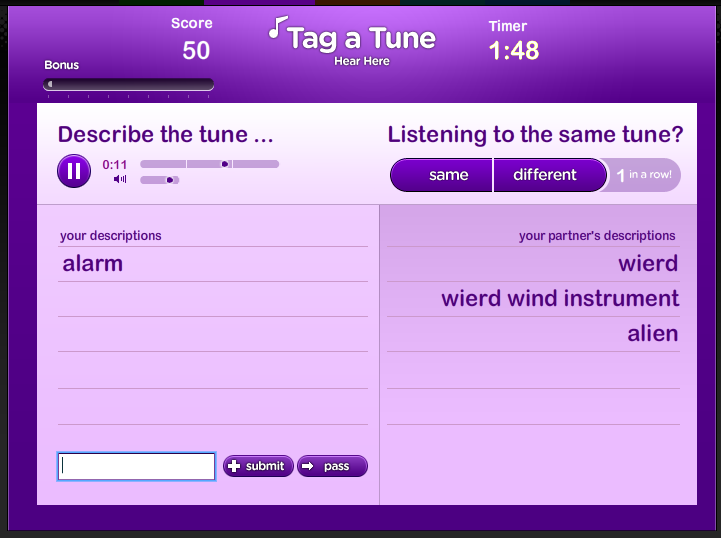
\includegraphics[scale=0.5]{Figures/tagatune.png}
    \rule{20em}{0.5pt}
  \caption[TagATune]{The user interface of \textit{TagATune}.}
  \label{fig:Tagatune}
\end{figure} 

\subsection{Co-Occurence Analysis}
The main idea behind co-occurence analysis is that two items that frequently co-appear in some kind of music-related document are similar. Data sources on which this kind of analysis is performed are typically music playlists \cite{pachet01} (compilation discs, radio stations or even simply users' playlist), music collections shared on peer-to-peer networks \cite{whitman02}, as well as web-pages \cite{zadel04} \cite{cohen00} and microblogs \cite{schedlmicro} \cite{zangerle12}. On microblogs, hashtags such as \texttt{#nowplaying} or \texttt{#music} are used to identify the individual listening events of a user and therefore building a simple user model. Co-occurence analysis with music playlists is commonly used in music recommendation system, while the same kind of analysis with web-pages is not common as Vector Space Models have yielded better results on the same kind of data \cite{schedlpohle}.

\section{Audio Content Analysis}
The main idea behind this kind of analysis is to directly extract useful information, through some algorithms (or library of algorithms), from the audio signal itself. The type of content information extracted may greatly vary in relation to the need of the research, but we can mainly distinguish four categories \cite{bogdanov13}:
\begin{itemize}
\item \textit{Timbral} information: related to the overall quality and color of the sound. There is not a general definition for music timbre; in \cite{orio06}, Orio has defined it as \textit{``the acoustic feature that is neither pitch nor intensity''}. In other words, timbre embraces all the features that make a C4 played by a violin sound clearly different from the same note played by a piano.
\item \textit{Temporal} information: related to rhythmic aspects of the composition, such as tempo or length of measures.
\item \textit{Tonal} information: directly linked to the frequency analysis of the signal and to the pitch. It can describe \texit{what notes are being played} or the tonality of a given track.
\item \textit{Inferred semantic} information: information inferred (usually through machine learning techniques) from the previous categories, in the attempt of giving a more defined and understable shape to the data collected. This kind of information may include descriptors such as genre, valence or arousal.
\end{itemize}

Information extracted through this family of techniques may also be categorized in the following way:
\begin{itemize}
\item Low-level data: information that has no musical meaning and that, more in general, is not interpretable by humans. Examples of this kind of descriptors are Mel Frequency Cepstral Coefficients (MFCCs) and Zero Crossing Rate (ZCR).
\item Mid-level data: information that has musical meaning but that is related to low-level music features. This kind of category mainly includes temporal and tonal descriptors. 
\item High-level data: corresponding to inferred semantic information.
\end{itemize}

Many of the studies conducted on the computation of music similarity through audio content descriptors have solely focused on low-level and timbral information, because this has been proved to bring alone to acceptable results with proper similarity measures \cite{mirage07}. However, more recent studies have shown some evidence of advantages in using high-level descriptors \cite{barrington07} \cite{west07} and, more in general, the most performant systems use data from all of these categories. When computing low and mid-level descriptors, the procedure requires the following operations:
\begin{itemize}
\item Conversion of the signal from stereo to mono, in order to compute all the descriptors for just one signal
\item Down-sampling of the signal to improve the performance while computing the descriptors
\item Segmentation of the signal into frames, short segments (usually from 512 to 2048 audio samples). Consecutive frames are usually not disjoint: the so-called \textit{hop-size} determines the hop of samples between the beginning of a frame and the next one, and is normally half or a quarter as big as the \textit{frame size}.
\item Computation of Fast Fourier Transform, with an appropriate prior windowing technique \footnote{Although this last step may not be strictly seen as a necessary operation, many descriptors rely on frequency analysis of the signal and therefore they require the computation of the Fourier Transform.}.
\end{itemize}

% Definition of blocks:
\tikzset{%
  block/.style    = {draw, thick, rectangle, minimum height = 3em,
    minimum width = 3em},
  sum/.style      = {draw, circle, node distance = 2cm}, % Adder
  input/.style    = {coordinate}, % Input
  output/.style   = {coordinate} % Output
}

\begin{figure}\hskip -1cm
\begin{tikzpicture}[auto, thick, node distance=2cm, >=triangle 45]
	\draw
	% Drawing the blocks
	node at (0.5,-0.8)[align=center][block] (stereotrack) {Stereo \\ Track}
	node at (4.8,-0.8)[align=center] [block] (monotrack) {Mono \\ Track}
	node at (10.4,-0.8)[align=center][block] (downsampled) {Downsampled\\ Signal}
	node at (15.6,-0.8)[align=center][block] (frames) {Frames}	
	;
    % Joining blocks. 
	\draw[->](stereotrack) -- node[align=center]{$conversion$ $to$\\$mono$ $signal$}(monotrack);
 	\draw[->](monotrack) -- node[align=center] {$downsampling$} (downsampled);
 	\draw[->](downsampled) -- node[align=center] {$decomposition$\\$into$ $frames$} (frames);

	% Boxing and labelling
	\draw [color=gray,thick](-0.5,-2.5) rectangle (16.6,1);
	\node at (-0.5,1) [above=5mm, right=0mm] {\textsc{Preliminary steps}};
\end{tikzpicture}
\caption{Standard procedure preliminary to the extraction of audio features.}
\label{fig:extraction}
\end{figure}

The computation of descriptors is then performed on each frame, and finally a single value for each descriptor is computed by the means of specific statistical analysis. Mean, median, variance and covariance are the most used statistical tools for calculating representative global values out of the enormous \textit{pool} of values computed in each frame.\\
Some more operations may sometimes be needed, such as de-noising \footnote{A set of operations which purpose is to reduce the amount of background noise in a signal, therefore incrementing the \texit{signal-to-noise ratio} (\textit{SNR} or sometimes \textit{S/N}).} of time-scaling of the signal. In the next sections, a more detailed look among most important descriptors will be given.

\subsection{Low-level Descriptors}
\subsubsection{MFCC}
Mel-Frequency Cepstral Coefficients (MFCCs) are a set of descriptors that have been widely used in MIR. They have been introduced in \cite{davis80} for speech recognition: since then, they are used in state of the art systems for speech recognition; furthermore, they have shown prominent results on music similarity systems when a single or multivariate Gaussian distribution is computed over their values. \\MFCCs are strongly related to human auditory system behaviour, which can be modeled by a set of critical bandpass filters (called \textit{``auditory filters''}) with overlapping bands, as already shown by Hermann von Helmholtz in 1863. The term \textit{critical band} was introduced by Harvey Fletcher in the 1940s, and indicates a range of frequencies around a specific one that may be not perceived in a totally independent way if played together to this reference frequency. This phenomenon is due to the inner behaviour of the cochlea, the sense organ of hearing within the inner ear. The mel bands are a set of bands that try to replicate auditory filters and therefore to somehow capture relevant features in the perception of music. Mel bands are based on the mel frequency scale, a perceptual scale of pitches judged by listeners to be equal in distance from one another. Mel frequency scale is linear at low frequencies (below 1000Hz) and logarithmic above. A popular formula from converting from $f$ Hertz to $m$ mels is:

\begin{equation}
m = 2595\log_{10}\left(1 + \frac{f}{1000} \right)
\end{equation}

Though a standard procedure for computing MFCCs values is not present, the following steps are generally performed:
\begin{enumerate}
\item Computation of Fourier Transform of the signal (of the frame)
\item Mapping of the powers obtained in step 1 onto mel bands. We then compute the logarithm of each power for each mel band.
\item Computation of the discrete cosine transform of these logarithm values.
\item Extraction of the MFCCs as amplitudes of the resulting spectrum. 
\end{enumerate}
Differences in the procedure often involve the shape of the windows used for mapping the spectrum into these bands, the choice of pre-filtering of the signal after step 1 or even the total number of MFCCs to extract. 

\subsubsection{Bark Bands}
The Bark scale, proposed by Eberhard Zwicker in 1961, is a psychoacoustical scale that tries to improve the mel scale, where each ``Bark'' stands for one critical bandwidth. Bark bands are 24, and are described as bands over which masking phenomenon and the shape of cochlea filters are invariant, which is strictly not true. To convert a frequency from $f$ Hertz to $B$ Barks we can use the formula:
\begin{equation}
B = 13a\tan \left(\frac{f}{1315.8} \right) + 3.5a\tan \left( \frac{f}{7518} \right)
\end{equation}

The published Bark bands (given in Hertz) are\footnote{\url{https://ccrma.stanford.edu/~jos/bbt/Bark_Frequency_Scale.html}}:\\ \\
\hfill\begin{minipage}{\dimexpr\textwidth-1.5cm}
[0, 100, 200, 300, 400, 510, 630, 770, 920, 1080, 1270, 1480, 1720, 2000, 2320, 2700, 3150, 3700, 4400, 5300, 6400, 7700, 9500, 12000, 15500]
\xdef\tpd{\the\prevdepth}
\end{minipage}

with corresponding band centers at:\\ \\
\hfill\begin{minipage}{\dimexpr\textwidth-1.5cm}
[50, 150, 250, 350, 450, 570, 700, 840, 1000, 1170, 1370, 1600, 1850, 2150, 2500, 2900, 3400, 4000, 4800, 5800, 7000, 8500, 10500, 13500]
\xdef\tpd{\the\prevdepth}
\end{minipage}
\\ \\
Again it can be seen that width of frequency bands grows slowly below 1000Hz, while showing the opposite behaviour at higher frequencies. 

\subsection{Mid-level Descriptors}
\subsubsection{Rhythm}
In traditional music notation, there are several notations for tempo. It may be expressed in BPM (beats per minute), MPM (measures per minute; commonly used in ballroom dance music) or by semantic notations indicating a range of BPM; an example of this last category of notations may be the popular system of Italian markings, such as \textit{presto} (168-200 BPM), \textit{andante} (84-90 BPM) or \textit{allegro} (120-128 BPM). \\ In the field of MIR, accurate notations are needed, therefore semantic annotations are disregarded in favour of more precise notation such as BPM and Onset Rate (OR).
\\ \\ 
\textbf{Onset Rate} \\ 
Onsets are generally defined as the beginning of a new musical note, and onset rate is therefore defined as the number of onsets in a time interval. This definition however hides several difficulties: several instruments might have a long attack time, therefore it is not trivial to determine the actual beginning of the note. Furthermore, in polyphonic music nominally simultaneous notes may be spread over tens of seconds, making this definition more blurred \cite{dixon06}. 
\begin{figure}[h]
\begin{center}
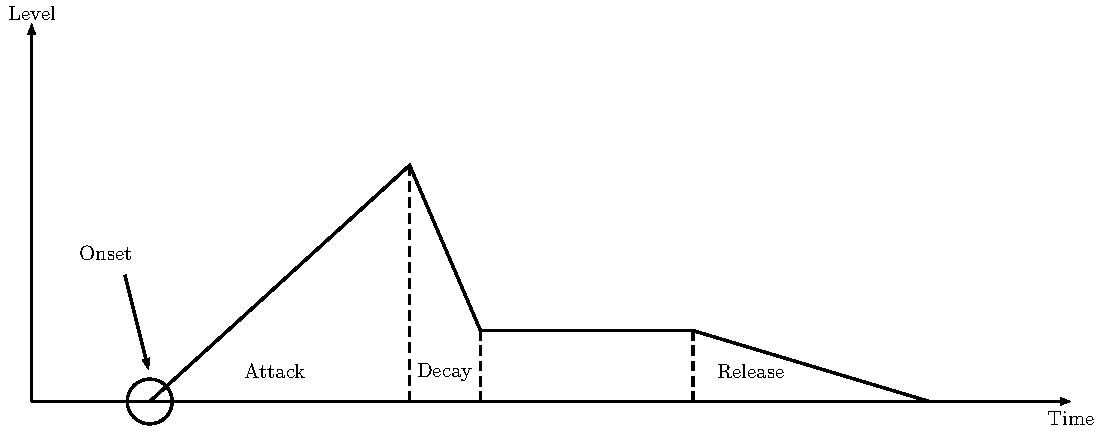
\includegraphics[scale=0.75]{Figures/onsets.pdf}
    \rule{20em}{0.5pt}
  \caption[Onset and sound envelope]{Onset and sound envelope.}
  \label{fig:GStreamer}
\end{center}
\end{figure} \\
Several ways of computing an onset detection function have been proposed, according to what aspects are taken into account for defining an onset. Actually, onset detection may be performed in time domain (when looking for significant changes in the overall energy), frequency domain (if looking for events regarding just a specific range of frequencies), phase domain or complex domain. 
Important algorithms for this task are:
\begin{itemize}
\item \textit{HFC}, the High Frequency Content detection function that looks for important changes on highest frequencies. It is very useful for detecting percussive events.
\item Spectral Flux, that decomposes the entire audible range of frequencies (approxitamely the interval 20-20000 Hz) into bins, measures changes in magnitude in each bin, and then sums all the positive changes across all the bins.
\item the Complex-Domain spectral difference function \cite{bello04} taking into account changes in magnitude and phase. It emphasizes note onsets either as a result of significant change in energy in the magnitude spectrum, and/or a deviation from the expected phase values in the phase spectrum, caused by a change in pitch.
\end{itemize}  
HFC was proposed by Masri in \cite{masri96}. Given the short-time Fourier transform (STFT) of the signal $x(n)$:\\
\begin{equation}
X_k(n) = \sum\limits_{m=-\frac{N}{2}}^{\frac{N}{2}-1} x(nh + m)w(m)e^{-\frac{2j\pi mk}{N}}
\end{equation}
(where $w(m)$ is again an $N$-point window, and $h$ is the hop size, or time shift, between adjacent windows), the idea behind HFC is to give more weight to higher frequencies, by defining a onset function whose values are computed in the follwing way:
\begin{equation}
HFC(n) = \frac{1}{N}\sum\limits_{k=-\frac{N}{2}}^{\frac{N}{2}-1} k\abs{X_k(n)}^{2}
\end{equation}

The HFC function produces sharp peaks during attack transients and is notably successful when faced with percussive onsets, where transients are well modeled as bursts of white noise \cite{bello05}.\\
On the other hand, the Spectral Flux $SF$ function is defined as follows:
\begin{equation}
SF(n) = \sum\limits_{k=-\frac{N}{2}}^{\frac{N}{2}-1} H(\abs{X(n, k)} - H(\abs{X(n - 1, k)})
\end{equation}
where $H = \frac{x + \abs{x}}{2}$ is the half-wave rectifier function. This algorithm greatly characterizes changes in magnitude spectrum but it quite weak to frequency-modulation phenomena (such as vibrato). To this end, the recently proposed variant SuperFlux \cite{bock13} seems to achieve much better results. \\
Another interesting onset function is the \textit{Complex Domain}, that calculates expected the expected amplitude and phase of the current bin $X(n, k)$ based on the previous two bins $X(n - 1, k)$ and $X(n -2, k)$. By assuming constant amplitude the expected value $X_T(n, k)$ is then computed:
\begin{equation}
X_T(n, k) = \abs{X(n - 1, k)}e^{\psi (n - 1, k) + \psi ' (n - 1, k)} 
\end{equation}
and therefore a complex domain onset detection function CD can be defined as the sum of absolute deviations from the target values \cite{dixon06}:
\begin{equation}
CD(n) = \sum\limits_{k=-\frac{N}{2}}^{\frac{N}{2}-1} \abs{X(n, k)-X_T(n,k)}
\end{equation}

Given an onset function (for instance one of the already cited $HFC(n)$, $SF(n)$ or $CD(n)$), onsets are then extracted by a peak-picking algorithm which finds local maxima in the detection function, subject to various constraints. Threshold and constraints used in the peak-picking algorithm has a large impact on the results, specifically on the ratio of false positives\footnote{True onsets that are not detected by the algorithm.} to false negatives\footnote{Points that are classified as onsets by the algorithm, while they are actually not.}. For instance, a higher threshold may lead to a lower number of false negatives but to a higher number of false positive, while a lower threshold may have the opposite effect. A compromise, mostly specific to the application, has to been found.
\\ \\ 
\textbf{BPM} \\ 
We can roughly define beats as those instants in which we tap with a foot while listening to track; beats therefore correspond to moments of musical emphasis in an audio signal. The algorithms for detecting the beats-per-minute (generally called \textit{beat tracking algorithms}) greatly rely on onset detection funcions. The basic idea is to look for some time-pattern that may explain the distribution of onsets over time, and hence derive BPM. They usually require more than one onset detection function to achieve good results. One of the beat tracking algorithm achieving very high reliability is TempoTapDegara, presented by N. Degara et al. in \cite{degara12}. This algorithm models the time between consecutive beat events and exploits both beat and non-beat signal observations, estimating not only beats position but also the expected accuracy. It specifically analyzes the input music signal and extracts a beat phase\footnote{The location of a beat with respect to the previous beat.} and a beat period salience observation signal, and then computes the beat period\footnote{Regular amount of time between beat events.} from these values.\\ The beat tracking probabilistic model then takes as input parameters the phase observation signal and the beat period estimation, returning the set of beat time estimates. The quality of the beat period salience observation signal is finally assessed and a $k$-nearest neighbor algorithm is used to measure the reliability of the beat estimates. \\
A \textit{complex spectral difference} method is used for computing the beat phase observation signal that will allow to compute all the other features. This onset function has shown good behavior for a wide range of audio signals and has been used with satisfying results in other beat tracking systems \cite{davies07}. 

\subsubsection{Tonality}
Many efforts have been taken in order to improve the techniques for detecting tonality or harmonic content of a song, as this is one of the most main aspects of western music (a direct consequence of tonality is the detection of predominant melody; to understand why this is so important just try to think how many times you whistled or sang a song to let other people recognize it). Many studies have focused on this aspect of music were not oriented toward the computation of similarity between tracks, but instead toward different tasks, such as \textit{automatic trascription of a polyphonic audio signal} (mainly into a MIDI representation) and \textit{source separation}, that is the task of isolating a single and specific instrument among many playing together. \\
From a music point of view, in western music an octave is made of 12 different pitches, and seven differents notes take place in this discrete range. According to the pitch assigned to each note, we may have different \textit{keys}, that are a combination of a \textit{tonic} (the central pitch) and the mode. \textit{Major} and \textit{minor} are the most popular modes. 
\begin{figure}[h]
\begin{center}
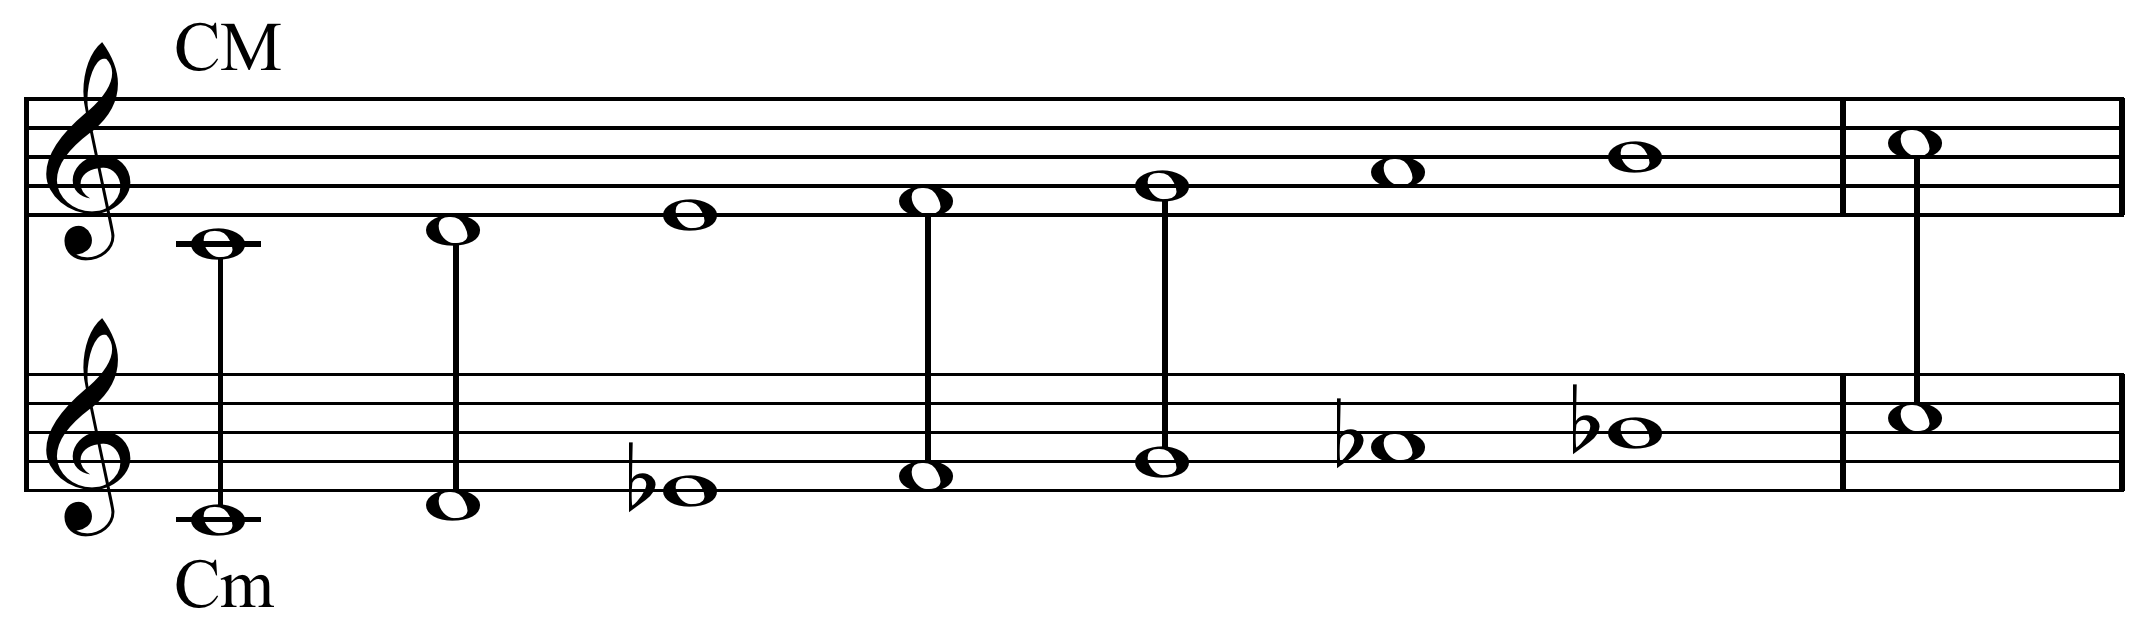
\includegraphics[scale=0.15]{Figures/majorminor.png}
    \rule{20em}{0.5pt}
  \caption[Major and minor modes]{Major and minor modes of C.}
  \label{fig:GStreamer}
\end{center}
\end{figure} \\
\textit{Harmony} is a term that denotes the simultaneous combination of notes, called \textit{chords}, and over time, \textit{chord progressions}.  One of the most important descriptor for extracting information related to tonality is called Harmonic Pitch Content Profile (\textbf{\textit{HPCP}}, also called chromagram). This is directly related to tonality and chord detection: chords can be recognized from from the \textit{HPCP} without even precisely detecting what notes are being played, and tonality can also be inferred by \textit{HPCP} (and in this case a previous estimation of chords is not necessary). \\
An \textit{HPCP} is a $12k$ size vector indicating the level energy for each profile class. If $k=1$, the \textit{HPCP} represents the intensities of the twelve semitone pitch classes, otherwise of subdivision of these\footnote{It may be extremely useful to study subdivision of semitone pitch classes when dealing with non-chromatic scales, that are very popular in eastern music.}. In \cite{gomez06}, Gómez proposes to distinguish tonality features on temporal scales: 
\begin{itemize}
\item Instantaneous: features attached to an analysis frame.
\item Global: features related to a wider audio segment, for instance a phrase, a chorus or the whole song.
\end{itemize}
Furthermore, Gómez proposes to split tonal descriptors in both low-level and high-level descriptors. We hence obtain the representation of tonal descriptors shown in Table \ref{table:tonaldescriptors}.
\begin{table}[h]
\begin{center}
\begin{tabular} { l l l }
\hline
Name         & Temporal Scale & Level of abstraction \\ \hline
HPCP         & Instantaneous  & Low                  \\ 
Chord        & Instantaneous  & High                 \\ 
Average HPCP & Global         & Low                  \\ 
Key          & Global         & High                 \\ \hline
\end{tabular}
\caption[Main tonal descriptors]{Main tonal descriptors.}
\label{table:tonaldescriptors}
\end{center}
\end{table}

The general approach for computing \textit{HPCP} can be summarized as follows:
\begin{itemize}
\item At first, some pre-processing of the audio signal may be performed. For instance, a transient detection algorithm may be used to detect and eliminate regions where the harmonic structure is noisy. This step is usually performed to decrease the computational cost of the \textit{HPCP} without affecting its output \cite{bonada00}.
\item At this point, spectral analysis is required: once the signal is segmented into frames of a proper size and a windowing function is applied, the Fast Fourier Transform (\textit{FFT}) is computed to get the frequency spectrum. Frames should not be too short, in order to have a better frequency resolution. 
\item A peak-picking algorithm is run to find those frequencies corresponding to local maxima in the spectrum. Usually, these algorithms are not run only on the interval [100, 5000] Hz: this has shown much better results, because outside this range the signal is predominantly noisy, due to some percussion and instrumental noise \cite{gomez06}.
\item The \textit{HPCP} is finally computed; many approaches have been developed for this task, all based on the pitch content profile algorithm presented by Fujishima in \cite{fujishima99}. At first, a mapping of each frequency bin of the \textit{FFT} to a pitch class is needed (for instance, \textit{FFT} bins corresponding to frequencies like 430Hz, 432Hz or 444Hz are mapped to the A at 440Hz). Then, the amplitudes inside each region are summed up and divided by the number of bins inside that region. Finally, the bins obtained are collapsed, so that bins referring to the same note but in a different octave (for example A4 and A5) are collapsed in a single bin for that note, indicating the overall energy of it in the frame. The \textit{HPCP} is different from the PCP in the sense that a higher resolution may be used for \textit{HPCP} bins (decreasing the quantization level to less than a semitone) and a weight function is introduced into the feature computation. The \textit{HPCP} value of the $n$-th \textit{HPCP} bin is calculated as:
\begin{equation}
HPCP(n) = \sum\limits_{i=1}^{nPeaks} w(n, f_i)a_i^2
\end{equation}
where $a_i$ and $f_i$ are respectively the magnitude and the frequency of the $i$th peak, $nPeaks$ is the number of spectral peaks considered, and $w(n, f_i)$ is the weight of the frequency bin $f_i$ when considering the \textit{HPCP} bin $n$.
\\ The performance of the \textit{HPCP} builder strongly relies on the weight function \cite{cabral05}. Note that, for how the common procedure of building \textit{HPCP} is defined, \textit{HPCP} are usually considered robust to noise and different tuning references. \\
\textit{HPCP} values are usually normalized in order to store the relative importance of the $n$th \textit{HPCP} bin:
\begin{equation}
HPCP_{normalized}(n) = \frac{HPCP(n)}{Max_n(HPCP(n))}
\end{equation}
\end{itemize}

Once the \textit{HPCP} are computed, additional tonal features may be computed, such as tonality or chords. Regarding tonality estimation, this is generally computed through a correlation analysis between the \textit{HPCP} obtained and a matrix of \textit{HPCP} profiles corresponding to different keys. 

\subsection{High-level Descriptors}

\subsection{Main Tools For Extracting Audio Content}
Many tools are available for the extraction of audio content descriptors from an audio signal. Many of them have been developed by researchers following the research necessities of MIR. This great variety of tools offers support to several operative systems (mainly Linux, Mac OS X and Windows) and programming languages (Java, C++, C, Python, Matlab). Some of this tools may be offered as standalone software or as a Vamp plugin. Not all the tools for extracting audio content are open-source, therefore not being particularly useful for the research community. In the following paragraphs, we'll briefly show the features of the tools taken into account on the development of this work.


\subsubsection*{Essentia}
\begin{figure}[h]
\begin{center}

\includegraphics[scale=0.95]{Figures/essentia.png}\\
    \rule{15em}{0.5pt}
  \caption[Essentia]{Essentia Logo.}
  \label{fig:Essentia}
\end{center}
\end{figure} \\
Essentia\footnote{\url{http://essentia.upf.edu/}} is an open-source C++ library of algorithms for audio analysis and audio-based music information retrieval. It has been developed at Music Technology Group\footnote{\url{http://mtg.upf.edu/}}, Universitat Pompeu Fabra, and has released under the Affero GPL license\footnote{\url{http://www.gnu.org/licenses/agpl.html}}. In its current version 2.0.1, it contains a large collection of spectral, temporal, tonal, and high-level music descriptors, algorithms for audio input/output functionality, standard digital signal processing blocks and statistical tools. The library can be complemented with Gaia \footnote{\url{https://github.com/MTG/gaia}}, a C++ library to apply similarity measures and classifications on the results of audio analysis. Both these libraries include Python 2.* bindings and support Linux, Mac OS X and Windows. Essentia has been in developed for over 7 years, incorporating the work of more than 20 researchers and developers through its history. \\
It offers two different modes: standard and streaming, the first being imperative while the latter being declarative. Each processing block is offered as an algorithm, and has three different types of attributes: inputs, outputs and parameters. Different blocks may be linked in order to perform the required processing task. In figure INSERT FIGURE a block diagram of a processing task is shown, composed of several different algorithms linked together. See Appendix A for consulting the full list of descriptors provided by Essentia 2.0.1.


\subsubsection*{The Echo Nest}
\begin{figure}[h]
\begin{center}

\includegraphics[scale=0.75]{Figures/echonest.jpg}
    \rule{20em}{0.5pt}
  \caption[Echo Nest]{Echo Nest logo.}
  \label{fig:Essentia}
\end{center}
\end{figure} \\
\textit{The Echo Nest}\footnote{\url{http://the.echonest.com/}} is a company that provides access, through Web API, to a collection of audio descriptors for a catalogue of over 36 million songs and almost 3 million artists. In order to access to this database, an API key is required, and some rate limits are imposed to the use of a free license (for instance, the maximum number of HTTP calls for minute is subject to a limit, generally 20). Users can decide to upload their collection into this database, so that descriptors will be computed for new songs and made available to other users. The performance of this library greatly depends on the chance that a song that is about to be analyzed has already been uploaded into this service. If this is not the case, the upload time has to be taken into account for performing the analysis task. \\ 
\textit{The Echo Nest} provides a great amount of descriptors for each track (see appendix~\ref{AppendixB} for the entire list), ranging from very accurate audio content information to metadata, and has been used by several commercial solutions, developed by \textit{Spotify}, \textit{Rdio}, \textit{Warner Music Group} and many others. Many official and unofficial libraries provide access to \textit{The Echo Nest} service; among these, the most important one is probably the official Python library \textit{Pyechonest}\footnote{\url{http://echonest.github.io/pyechonest/}}, that provides full access to all of the Echo Nest methods including artist search, news, reviews, blogs, similar artists as well as methods for retrieving detailed analysis information about an uploaded track. Furthermore, the library \textit{Echo Nest Remix\footnote{\url{http://echonest.github.io/remix/}}} worths mentioning, as it is a library for audio manipulation and mixing and has been used by many \textit{web-applications}, including The Infinite Jukebox. \\
However, the source code of \textit{The Echo Nest} API service is not provided, therefore it has little usefulness to the research community. \\ \textit{The Echo Nest} has been aquired by \textit{Spotify} on March 2014.


\subsubsection*{jMIR}
jMir\footnote{\url{http://jmir.sourceforge.net/}} is an open-source software suite implemented in Java and intended for use in music information retrieval research. Its development has been guided by Cory McKay (Marianopolis College), with many researchers from several institutions contributing to it. \textit{jMir} is composed of several components differentiated in their scope, spacing from audio content analysis (performed by \textit{jAudio}), to web mining of metadata and machine learning algorithms for classification. \\ The most relevant components of this suite are as follows:
\begin{itemize}
\item \textit{ACE}: Pattern recognition software that utilizes meta-learning. 
\item \textit{jAudio}: Software for extracting low and high-level features from audio recordings.
\item \textit{jSymbolic}: Software for extracting high-level features from MIDI recordings.
\item \textit{jWebMiner}: Software for extracting cultural features from web text
\item \textit{jSongMiner}: Software for identifying unknown audio and extracting metadata about songs, artists and albums from various web services.
\end{itemize}


\subsubsection*{MIRtoolbox}
MIRtoolbox\footnote{\url{https://www.jyu.fi/hum/laitokset/musiikki/en/research/coe/materials/mirtoolbox}} is a set of functions for Matlab, dedicated to the extraction of audio content features from audio files. The design is based on a modular framework: algorithms are decomposed into stages, formalized using a minimal set of elementary mechanisms, with the objective of offering an overview of computational approaches in the MIR research field. MIRtoolbox has been developed at the Jyväskylän Yliopisto (University of Jyväskylä, Finland), by Olivier Lartillot, Petri Toiviainen and Tuomas Eerola.


\section{Computing Music Similarity with Audio Content Descriptors}
\label{sec:audiocontentsimilarity}

\subsection{Notable studies on large databases}
When large music collections are used, performance of similarity computation algorithms become critic. Although the collection to be used by the system during its public use can't be considered large, the necessary decomposition of it into hundred of thousands excerpt to be analyzed just in few seconds makes performance a critical factor when designing and implementing an algorithm. Therefore, a deep look into studies where large collections were used was needed.\\
The first content-based music recommendation system working on large collections (over 200,000 songs) was published by Cano et al. in \cite{cano05}, 2005. The system presented on this work relies on rhythmic and timbre features, combined to form a music similarity feature vector. No special indexing technique was used. \\
The first music recommendation system for large databases using Gaussian timbre features was proposed some months later by Roy et al. in \cite{roy05}. In this work, they propose to use a Monte-Carlo approximation of the Kullback-Leibler (KL) divergence to measure music similarity. The method proposed is, in principle, similar to the one proposed by Schnitzer et al. in \cite{fastmap12}, which has been used on the development of this thesis work (see \ref{sec:fastmap}). To pre-filter their results, Roy et al. increase the sampling rate of the Monte-Carlo approximation. As the divergence values converge, they are able to reduce the number of possible nearest neighbors. This method has shown good performance, both in query time and results.\\
A different attempt of improving performance was proposed by Levy and Sandler in \cite{levy06} where they use only diagonal covariance matrix instead of a full one to compute music similarity. While this has shown a ten-fold speedup compared to the full Kullback Leibler divergence, the quality of this simpler similarity measure results in worse genre classification rates. 


\section{Conceptual Differences Between Metadata and Audio Content Information}
The performance of content-based approaches is considerably lower \cite{slaney2011}.
It is challenging to try to make the so-called \textit{semantic gap} smaller \cite{aucou2009}

The advantage of relying on the audio signal over, say, expert annotations, is that
the process is objective and can be automated to a large extent. However, extracting
the features can be computationally costly \cite{schma13}. Another
limitation is that there might be features like the release date, the “freshness,” or
popularity of a track, which can be relevant in the playlist generation process but that
cannot be extracted from the audio signal \cite{celma08}.

When used in an automated process, data completeness and consistency are crucial.
Another potential problem is that not all types of metadata are objective, and annotations regarding, for example, the mood or the genre of a track can be imprecise or inconsistent \cite{celma2010}.

(speaking of tags) Although such annotations can be rich and diverse, the perception of music is again subjective and can even be influenced by the perception of other people \cite{mcdermott12}; tags only for popular songs \cite{celma2010}

When dealing with track ratings: grabbed from a wall posting on Facebook \cite{germain13} or a tweet on twitter \cite{hauger13}, 1-to-5 rating scales like on iTunes. Challenges: problem of data sparsity (especially for the tracks from the long tail), a positivity bias (the phenomenon that most of the ratings are highly positive and negative feedback is rare \cite{celma2010}).